% main.tex
% header.tex
\documentclass[a4paper,11pt,twoside,ngerman,color]{book}
\usepackage[a4paper,left=3.5cm,right=2.5cm,bottom=3.5cm,top=3cm]{geometry}

\usepackage[german,english]{babel}

\usepackage[pdftex]{graphicx,color}
\usepackage{amsmath,amssymb,subfigure}


% Theorem-Umgebungen
\usepackage[amsmath,thmmarks]{ntheorem}

% Korrekte Darstellung der Umlaute
\usepackage[utf8]{inputenc}
\usepackage[T1]{fontenc}

% Algorithmen
\usepackage[plain,chapter]{algorithm}
\usepackage{algpseudocode}
%\usepackage{algorithmic}
%\usepackage[english]{algorithm2e}


\usepackage{enumerate}

%\usepackage[parfill]{parskip}

% Bibtex deutsch
\usepackage{bibgerm}

% URLs
\usepackage{url}

\usepackage{minted}

% Caption Packet
\usepackage[margin=0pt,font=small,labelfont=bf]{caption}
% Gliederung einstellen
%\setcounter{secnumdepth}{5}
%\setcounter{tocdepth}{5}

% Theorem-Optionen %
\theoremseparator{.}
\theoremstyle{change}
\newtheorem{theorem}{Theorem}[section]
\newtheorem{satz}[theorem]{Satz}
\newtheorem{lemma}[theorem]{Lemma}
\newtheorem{korollar}[theorem]{Korollar}
\newtheorem{proposition}[theorem]{Proposition}
% Ohne Numerierung
\theoremstyle{nonumberplain}
\renewtheorem{theorem*}{Theorem}
\renewtheorem{satz*}{Satz}
\renewtheorem{lemma*}{Lemma}
\renewtheorem{korollar*}{Korollar}
\renewtheorem{proposition*}{Proposition}
% Definitionen mit \upshape
\theorembodyfont{\upshape}
\theoremstyle{change}
\newtheorem{definition}[theorem]{Definition}
\theoremstyle{nonumberplain}
\renewtheorem{definition*}{Definition}
% Kursive Schrift
\theoremheaderfont{\itshape}
\newtheorem{notation}{Notation}
\newtheorem{konvention}{Konvention}
\newtheorem{bezeichnung}{Bezeichnung}
\theoremsymbol{\ensuremath{\Box}}
\newtheorem{beweis}{Beweis}
\theoremsymbol{}
\theoremstyle{change}
\theoremheaderfont{\bfseries}
\newtheorem{bemerkung}[theorem]{Bemerkung}
\newtheorem{beobachtung}[theorem]{Beobachtung}
\newtheorem{beispiel}[theorem]{Beispiel}
\newtheorem{problem}{Problem}
\theoremstyle{nonumberplain}
\renewtheorem{bemerkung*}{Bemerkung}
\renewtheorem{beispiel*}{Beispiel}
\renewtheorem{problem*}{Problem}

% Algorithmen anpassen %
\renewcommand{\algorithmicrequire}{\textit{Eingabe:}}
\renewcommand{\algorithmicensure}{\textit{Ausgabe:}}
\floatname{algorithm}{Algorithmus}
\renewcommand{\listalgorithmname}{Algorithmenverzeichnis}
\renewcommand{\algorithmiccomment}[1]{\color{grau}{// #1}}

% Zeilenabstand einstellen %
\renewcommand{\baselinestretch}{1.25}
% Floating-Umgebungen anpassen %
\renewcommand{\topfraction}{0.9}
\renewcommand{\bottomfraction}{0.8}
% Abkuerzungen richtig formatieren %
\usepackage{xspace}
\newcommand{\vgl}{vgl.\@\xspace} 
\newcommand{\zB}{z.\nolinebreak[4]\hspace{0.125em}\nolinebreak[4]B.\@\xspace}
\newcommand{\bzw}{bzw.\@\xspace}
\newcommand{\dahe}{d.\nolinebreak[4]\hspace{0.125em}h.\nolinebreak[4]\@\xspace}
\newcommand{\etc}{etc.\@\xspace}
\newcommand{\evtl}{evtl.\@\xspace}
\newcommand{\ggf}{ggf.\@\xspace}
\newcommand{\bzgl}{bzgl.\@\xspace}
\newcommand{\so}{s.\nolinebreak[4]\hspace{0.125em}\nolinebreak[4]o.\@\xspace}
\newcommand{\iA}{i.\nolinebreak[4]\hspace{0.125em}\nolinebreak[4]A.\@\xspace}
\newcommand{\sa}{s.\nolinebreak[4]\hspace{0.125em}\nolinebreak[4]a.\@\xspace}
\newcommand{\su}{s.\nolinebreak[4]\hspace{0.125em}\nolinebreak[4]u.\@\xspace}
\newcommand{\ua}{u.\nolinebreak[4]\hspace{0.125em}\nolinebreak[4]a.\@\xspace}
\newcommand{\og}{o.\nolinebreak[4]\hspace{0.125em}\nolinebreak[4]g.\@\xspace}
\newcommand{\oBdA}{o.\nolinebreak[4]\hspace{0.125em}\nolinebreak[4]B.\nolinebreak[4]\hspace{0.125em}d.\nolinebreak[4]\hspace{0.125em}A.\@\xspace}
\newcommand{\OBdA}{O.\nolinebreak[4]\hspace{0.125em}\nolinebreak[4]B.\nolinebreak[4]\hspace{0.125em}d.\nolinebreak[4]\hspace{0.125em}A.\@\xspace}

% Leere Seite ohne Seitennummer, naechste Seite rechts
\newcommand{\blankpage}{
 \clearpage{\pagestyle{empty}\cleardoublepage}
}

% Keine einzelnen Zeilen beim Anfang eines Abschnitts (Schusterjungen)
\clubpenalty = 10000
% Keine einzelnen Zeilen am Ende eines Abschnitts (Hurenkinder)
\widowpenalty = 10000 \displaywidowpenalty = 10000
% EOF

\begin{document}
\selectlanguage{german}
\begin{titlepage}
\definecolor{TUGreen}{rgb}{0.517,0.721,0.094}
\vspace*{-2cm}
\newlength{\links}
\setlength{\links}{-1.5cm}
\sffamily
\hspace*{\links}
\begin{minipage}{12.5cm}

\includegraphics[width=8cm]{bilder/tud_logo_rgb}
%\hspace*{-0.25cm} \textbf{TECHNISCHE UNIVERSIT"AT DORTMUND}\\
%\hspace*{-1.2cm} \rule{5mm}{5mm} \hspace*{0.1cm} FACHBEREICH INFORMATIK\\
\end{minipage}

\vspace*{4cm}

\hspace*{\links}
\hspace*{-0.2cm}
\begin{minipage}{9cm}
\large
\begin{center}
{\Large Meisterarbeit} \\
\vspace*{1cm}
\textbf{Titel} \\
\vspace*{1cm}
Konstantin Tkachuk\\
% \vspace*{1cm}
Februar 2017
\end{center}
\end{minipage}
\normalsize
\vspace*{5.5cm}

% \hspace*{\links}

\vspace*{2.1cm}

\hspace*{\links}
\begin{minipage}[b]{5cm}
% \normalsize
\raggedright
Gutachter: \\
Prof. Dr.-Ing. Olaf Spinczyk\\
Dr. Sven Seiler \\
\end{minipage}

\vspace*{2.5cm}
\hspace*{\links}
\begin{minipage}[b]{8cm}
% \normalsize
\raggedright
Technische Universit"at Dortmund \\
Fakult"at f"ur Informatik\\
Lehrstuhl Informatik 12\\
http://ls12-www.cs.tu-dortmund.de
\end{minipage}
%%%%%%%%%%%%%%%%%%%%%%%%%%%%%%%%%%%%%%%%%%%%%%%%%%
% bei Kooperation mit anderen Lehrstuehlen,
% sonst weglassen
\begin{minipage}[b]{8cm}
% \normalsize
\raggedleft
In Kooperation mit:\\
Materna GmbH
\end{minipage}
%%%%%%%%%%%%%%%%%%%%%%%%%%%%%%%%%%%%%%%%%%%%%%%%%%

\end{titlepage}

\blankpage
\pagenumbering{roman}
%Vorwort
%\topskip0pt
%\vspace*{\fill}
\null\vfill
\begin{center}
	\subsubsection*{Zusammenfassung}
\end{center}
Abstract text
%\vspace*{\fill}
\vfill\null
\tableofcontents
\cleardoublepage
\pagenumbering{arabic}
% Kapitel
% einleitung.tex
\chapter{Einleitung}
\section{Motivation und Hintergrund}
Motivation und Hintergrund

\section{Ziele der Arbeit}
Ziel dieser Arbeit ist es die Welten von Smart Home und webbasierten Task Automation Services zusammen zu bringen. Es soll ein Demonstrator entwickelt werden, der die  Funktionalitäten beider Ansätze kombiniert und in einem gemeinsamen Kontext anbietet. Konkreter sind die Ziele in Sektion \ref{sec:ziele} erläutert.


\section{Aufbau der Arbeit}
Nach der Einleitung wird der aktuelle Stand der Forschung bezüglich \textit{Internet der Dinge}, \textit{SmartHome} und \textit{Task Automation Services} vorgestellt und die Ziele der Arbeit daraus abgeleitet. Daraufhin wird in Kapitel 3 das Framework Eclipse SmartHome (ESH) vorgestellt. In Kapitel 4 wird konkret betrachtet, wie die Funktionalitäten eines Task Automation Services in ESH integriert werden können.

Im folgenden Kapitel 5 wird die Implementierung des Entwurfs mit Hilfe von entsprechenden
Diagrammen vorgestellt. Der Quell-Code ist auf der mit der Arbeit mitgelieferten
CD einsehbar. Danach wird in Abschnitt 6 die Implementierung evaluiert. Schließlich folgt
noch eine kurze Zusammenfassung der geleisteten Arbeit und ein Ausblick auf mögliche
Weiterentwicklungen in Kapitel 7.


% kapitel2.tex
\chapter{Stand der Forschung}
In diesem Kapitel wird der aktuelle Stand der Forschung des Internets der Dinge erläutert. Es wird besonders auf die Themen Smart Home und Task Automation Services eingegangen, sowie darauf, welche Vorteile sich durch das Kombinieren dieser Ansätze erhoffen lassen.


\section{Internet of Things}
Die enorm steigende Anzahl von „intelligenten Gegenständen“ mit eingebetteten Computern, die den Menschen im alltäglichen Leben unterstützen sollen, hat zu der Prägung des Begriffs „Internet der Dinge“ (IoT) geführt. Jedes dieser Dinge hat seine eigene Funktionalität und im Verbund stellen sie eine große Menge an Daten zur Verfügung. Im Rahmen von zahlreichen Forschungsprojekten \cite{ierc:portfolios} werden Möglichkeiten untersucht, IoT mit unterschiedlichen Technologien zu kombinieren. Unter anderem werden Technologien, wie Cloud Computing, Machine-2-Machine Learning und Semantic Web kritisch betrachtet. Außerdem werden Kernprinzipien, wie Architektur und Standardisierung intensiv recherchiert. Sie werden in dedizierten Forschungsprojekten \cite{icore:achitecture}\cite{iota:d25} immer wieder aufgegriffen.

Im Laufe der Zeit haben sich verschiedene Aspekte des IoT herausgebildet, unter anderem das Smart Home.

\subsection{Smart Home}
Ein mit IoT eng verwobenes Thema ist das Smart Home\cite{SmartHomeIoT}, welches die elektronische Steuerung von ausgewählten Geräten mit z.B. einer Rule Engine kombiniert um eine Automatisierung des Geräteverhaltens in einem Zusammenspiel zwischen Sensorik und Aktortik zu erreichen. Smart Home grenzt sich von IoT ab indem es auf Sensoren und Aktoren spezialisiert ist, die im Kontext eines Hauses relevant sind.\\

Bis dato wurden zahlreiche Smart Home Lösungen von verschiedenen Anbietern entwickelt. Man kann prinzipiell zwei Arten von Lösungen unterscheiden. \textit{Proprietäre} Produkte (z.B. \textit{RWE SmartHome}\cite{RWE}) spezialisieren sich auf eine sehr begrenzte Anzahl von Geräten und bemühen sich maximale Unterstützung für diese Geräte zu bieten. Dies sorgt für eine Fragmentierung des Marktes. \textit{Open Source} Lösungen hingegen verfolgen das Ziel möglichst offen für verschiedene Geräte und Protokolle zu bleiben.\\ 

Da Open Source Lösungen aktuell noch aktiv in der Entwicklung sind und hauptsächlich als Software existieren, erfordert ihr Einsatz von Nutzern ein gewisses Maß an technischen Vorkenntnissen. In der Regel muss der Nutzer passende Hardware bereitstellen und die Software selbst installieren. Bei Problemen kann Support bestenfalls auf Foren von der Community gefunden werden. 

Diese Gründe führen dazu, dass Open Source Lösungen derzeit noch nicht massenhaft zum Einsatz kommen.



\subsection{Task Automation Services}
\label{subsec:tas}
Die Automatisierung von Aufgaben ist eins der zentralen Bestreben unseres alltäglichen Lebens. Es macht das Leben einfacher und erlaubt uns kostbare Zeit zu sparen. Ob Notifikation auf dem Smartphone, wenn eine Email eingeht oder das Einschalten von Lampen, wenn ein Raum betreten wird, solche Automatisierung ist heutzutage überall zu finden. Lange Zeit musste jede derartige Automatisierung einzeln entworfen, konfiguriert und implementiert werden. Doch die steigende Anzahl von intelligenten Gegenständen und die Allgegenwärtigkeit des Internets belassen dies der Vergangenheit. Nun hat sich der Ansatz der Task Automation Services\cite{ieee:tas} gebildet.

Ein Task Automation Service (TAS) ist ein Dienst, der es Endnutzern ermöglicht das Verhalten von verschiedenen Services und Geräten in eigenen Szenarien jederzeit selbst zu automatisieren. Solche Szenarien basieren auf Event-Condition-Action (ECA) Regeln\cite{ECA}, welche es ermöglichen, auf Events unter festgelegten Bedingungen mit entsprechenden Aktionen zu reagieren. Meistens wird dies durch  einen intuitiven visuellen Regel Editor ermöglicht.

%evtl näher eingehen, was typische Charakteristika von TAS sind: Channels, channel paradigms

Aktuell gibt es noch vergleichsweise wenige TAS. Ein Überblick über existierende  Services bietet Abbildung \ref{fig:tasoverview}.

\begin{figure}[h]
	\centering
	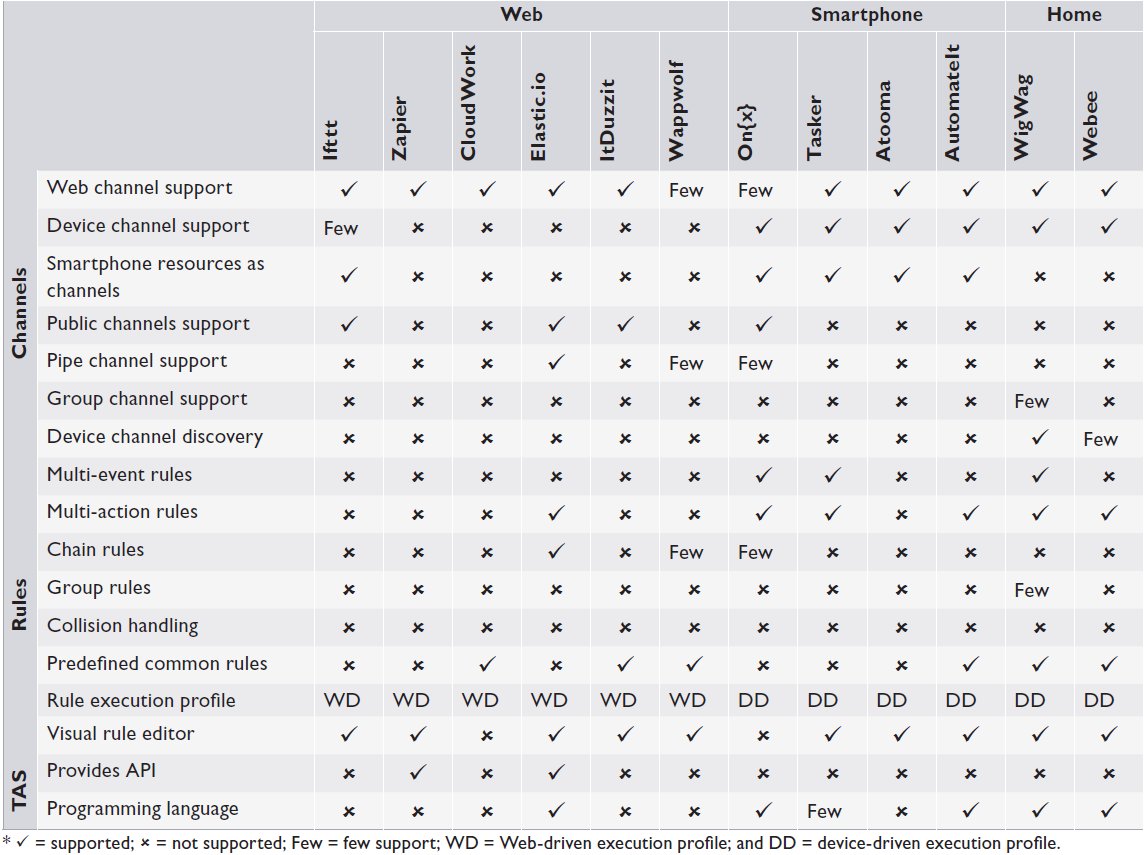
\includegraphics[width=\textwidth]{bilder/TASOverview}
	\caption{Überblick über existierende Task Automation Services \cite{ieee:tas}}
	\label{fig:tasoverview}
\end{figure}

Wie in der Abbildung zu sehen ist, gibt es unterschiedliche Ansätze. Einige TAS sind in der Cloud angesiedelt, was bedeutet, dass sie, sofern Internet verfügbar ist, jederzeit und von überall erreichbar sind. Die aktuell mächtigsten und bekanntesten TAS sind \textit{IFTTT} \cite{IFTTT} und \textit{Zapier}\cite{Zapier}. Sie unterstützen hunderte unterschiedlicher Web Services, bieten aber keine Möglichkeit mit Geräten direkt zu interagieren. Ihr Fokus ist es zu ermöglichen eine Vielzahl von Szenarien auf eine einfache Art und Weise zu erstellen. Auf komplexere Regeln und Szenarien sind ihre Rule Engines nicht ausgelegt. 
Um diese TAS zu nutzen, muss man jedoch bereit sein, sämtliche Zugriffsrechte, die für die zu automatisierenden Dienste (z.B. \textit{Facebook}, \textit{Twitter}, etc.) benötigt werden, dem Cloud Service anzuvertrauen.

Andere Task Automation Services arbeiten lokal auf Smartphones. Solche TAS konzentrieren sich auf die Automatisierung von den auf dem Gerät laufenden Services. Die Unterstützung von der Automatisierung von Web Services ist nur in dem Umfang gegeben, in dem diese Web Services direkten Kontakt mit dem Smartphone haben.  

Schließlich gibt es TAS, die auf einer dedizierten Basis im Haus arbeiten. Solche Task Automation Services konzentrieren sich auf die direkte Steuerung von Geräten mithilfe der entsprechenden Protokolle. Im Grunde sind sie äquivalent zu Smart Home. 

Im Rahmen dieser Arbeit wird Smart Home jedoch getrennt von TAS behandelt, da der Fokus der Automatisierung völlig unterschiedlich ist. Mehr dazu in Sektion \ref{sec:idee}.



\subsubsection{IFTTT}
Ein Beispiel für Task Automation Services in der Cloud ist IFTTT, welches eine große Anzahl verschiedener Services (\textit{Facebook}, \textit{Dropbox}, \textit{Philips Hue},   etc.) integriert und eine rudimentäre Rule Engine anbietet, die es erlaubt auf eine einfache Art und Weise serviceübergreifende „if this than that“ Anweisungen zu hinterlegen, die der klassischen „EDV“ ähneln. Es wird eine feste Trigger Komponente gewählt, die etwas auslöst, daraufhin wird die Aktion festgelegt, die ausgeführt werden soll. Solche Condition/Command Paare werden in IFTTT \textit{Recipes} genannt. 

Bis dato lassen sich komplexere Szenarien mit \textit{IFTTT} nicht abbilden.  Das bedeutet, dass es keine Möglichkeit gibt, beispielsweise, Und- und Oder-Bedingungen zu definieren, die es ermöglichen würden, mehrere Conditions in einem Recipe zu verknüpfen.

Ein weiterer Aspekt von IFTTT ist, dass es für die Anbindung von Services Zugriffsrechte auf sämtliche Accounts des Users bedarf. Aus einer Datenschutz-Perspektive\cite{cloudsec} stellt das ein Risiko für den Endnutzer dar, da seine sämtlichen Account-Daten an einer Stelle gesammelt sind. Im Falle einer Sicherheitslücke bei IFTTT wären alle damit gekoppelten Services in Gefahr. 

\section{Zentrale Idee}
\label{sec:idee}
Wie in Sektion \ref{subsec:tas} zu sehen ist, kann man drei prinzipiell unterschiedliche Arten von Task Automation Services unterscheiden: Cloud Service, Smartphone Applikation und Smart Home. Sie weisen zwar viele Gemeinsamkeiten auf, doch allein aus den Namen lässt sich ablesen, dass es sich dabei um grundlegend verschiedene Lösungen handelt. 

Die Cloud Services unterstützen nur begrenzt die \glqq direkte\grqq{}  Steuerung von Geräten. Außerdem sind die zum Einsatz kommenden Rule Engines sehr rudimentär. Smart Homes hingegen haben in der Regel mächtige Rule Engines und bieten die Möglichkeit komplexe Szenarien zu definieren. Zusätzlich sind sie in der Lage, Geräte direkt anzusteuern. Im Rahmen dieser Arbeit werden die Smartphone Applikationen nicht näher betrachtet.\\

Die zentrale Idee dieser Arbeit ist es ein Smart Home mit einem Cloud Service TAS zu verschmelzen. Dadurch soll ein Ganzes entstehen, welches mehr ist, als die Summe seiner Teile: Ein (Work-)Flow Automation Service im Kontext Smart Home (FLASH).

\subsection{Ziele}
\label{sec:ziele}
Ziel dieser Arbeit ist es die Welten von Smart Home und webbasierten Task Automation Services zusammen zu bringen. Durch die Integration mit Smart Home soll die direkte Steuerung von Geräten befähigt werden. Außerdem soll die Mächtigkeit der Smart Home Rule Engine genutzt werden, um komplexere Regeln und Szenarien zu ermöglichen. Schließlich sollen die Datenschutzprobleme gelöst werden, indem sämtliche Zugriffsdaten on-premise galagert und dadurch nie einem Risiko ausgesetzt werden.

Es soll ein Demonstrator entwickelt werden, der die Funktionalitäten von Smart Home und TAS kombiniert und in einer on-premise Anwendung anbietet. Hierzu soll das Eclipse SmartHome Framework als Basis verwendet und um Funktionalitäten von webbasierten TAS angereichert werden. Die entstandene Anwendung soll auf einem Raspberry Pi laufen.

Die entstandenen Funktionalitäten sollen anhand von einer Reihe von konkreten Services demonstriert werden. Unter anderem sollen ein Wetterdienst, ein Filesharing Service und ein Social Media Service angebunden werden. Die Zusammenarbeit dieser Services untereinander und mit Smart Home Geräten soll anhand von Beispiel-Regeln demonstriert werden. Außerdem soll es möglich sein neue Regeln zum System über eine Benutzeroberfläche hinzufügen zu können.

Zum Schluss soll der entstandene Demonstrator evaluiert werden. Es soll geprüft werden, inwiefern Task Automation Services als on-premise Lösung sinnvoll sind unter Betrachtung von Aspekten wie Reaktionszeiten und Netzwerklast. Hierzu soll ein Vergleich der erstellten Anwendung mit \textit{IFTTT} stattfinden.

\subsection{Konkrete Anforderungen}
\label{sec:anforderungen}
In dieser Sektion werden aus den oben genannten Zielen konkrete Anforderungen an den resultierenden Demonstrator abgeleitet und im Detail festgehalten.

Es wird erwartet, dass der Demonstrator folgende Eigenschaften erfüllt:
\begin{enumerate}
\item Der Demonstrator soll on-premise auf einem Raspberry Pi 3 Model B laufen.
\item Er soll intern wie eine Smart Home Zentrale agieren und in der Lage sein, Geräte innerhalb des Hauses auch ohne Internetverbindung steuern zu können.
\item Bei vorhandener Internetverbindung soll er in der Lage sein ausgewählte  webbasierte Dienste zu automatisieren.
\item Sämtliche (Zugriffs-)Daten sollen lokal auf dem Gerät gelagert werden. 
\item Die Webdienste sollen nahtlos in die Rule Engine integriert werden, sodass komplexe Szenarien ermöglicht werden.
\item Es soll eine grafische Benutzeroberfläche angeboten werden, in der der Nutzer in der Lage ist eigene Szenarien zur Laufzeit zu definieren.

\end{enumerate}

\subsubsection{Anzubindende Services}
\label{subsec:anzubindende_services}
Im Rahmen der Arbeit sollen folgende populäre Internetdienste in den Demonstrator exemplarisch integriert werden:
\begin{enumerate}
\item \textbf{Twitter}\cite{twitter} Der Demonstrator soll in der Lage sein für den Nutzer Tweets zu schreiben, sowie auf Tweets zu reagieren. Beispielsweise soll es möglich sein, Medien in Tweets automatisch in die Dropbox zu speichern.
\item \textbf{Dropbox}\cite{dropbox} Es soll möglich sein, automatisch Dateien in die Dropbox zu speichern, sowie auf das Ändern von existierenden Dokumenten zu reagieren.
\item \textbf{Wetterdienst}\cite{wetterapi} Es sollen Wetterdaten aus dem Internet bezogen und auf konkrete Wetterbedingungen reagiert werden können.
\item \textbf{Email} Der Demonstrator soll in der Lage sein an beliebige Adressen Emails zu versenden.
\end{enumerate}




% Ansatz.tex
\chapter{Eclipse Smarthome}
\label{chap:esh}
In diesem Kapitel wird Eclipse SmartHome vorgestellt. Es werden zunächst die grundlegenden Konzepte des Frameworks erläutert. Anschließend wird auf für die Arbeit relevante konkrete Aspekte näher eingegangen.

\section{Überblick}
Hier wird ein kurzer Überblick über Smarthome gegeben
- Was ist ESH?
- Zugrunde liegende Technologien
- Zentrale Features von ESH
- Wo kommt es zum Einsatz
-
Im folgenden werden die verschiedenen Aspekte von ESH erläutert.

\subsection{Bindings}
\subsection{Automatisierung}
\subsection{Deklarative Typen}
\subsection{Persistenz}

\section{Modell}
\subsection{Channels}
\subsection{Things und Bridges}
\subsection{Links}
\subsection{Items}
\subsection{Discovery und Inbox}

\section{Rule Engine}
\subsection{Triggers}
\subsection{Conditions}
\subsection{Actions}
\subsection{Events}

\section{Controller}
\subsection{Thing Handler}
\subsection{Trigger/Action Handler}

\section{Fazit}

\chapter{Entwurf}
\label{chap:entwurf}
In diesem Kapitel wird vorgestellt, wie die neuen Funktionalitäten in ESH integriert werden sollen.


\section{Webservices}
Man kann im Allgemeinen zwischen \textit{öffentlichen} und \textit{privaten} Webservices differenzieren. Der wesentliche Unterschied ist, dass öffentliche Dienste keine Nutzerverwaltung einschließen - sämtliche Schnittstellen und bereitgestellten Informationen sind frei verfügbar. Ein online Wetterdienst ist ein Beispiel für einen öffentlichen Webservice. 

Unter privaten Webservices handelt es sich in diesem Kontext um Dienste, deren Funktionalität von eingeloggten User abhängt. Ein Beispiel hierfür ist \textit{Dropbox}. Der Zugriff auf die in der Dropbox gelagerten Dateien ist erst möglich, nachdem sich der User im System authentisiert hat. 

Es gibt eine Vielzahl von verschiedenen Sicherheitsprotokollen, die an dieser Stelle zum Einsatz kommen. Vor allem hat sich derzeit das OAuth-Protokoll etabliert, welches auch in den Webservices \textit{Twitter} und \textit{Dropbox} genutzt wird.\\

\subsubsection{OAuth Standard}
OAuth ist ein offener Standard für Autorisierung, der es ermöglicht Nutzern Applikationen von Drittanbietern den Zugriff auf Webdienste in ihrem Namen zu gestatten, ohne dabei das eigene Passwort freizugeben. Dies geschieht in der Regel in mehreren Schritten.

\begin{enumerate}
\item Die Applikation registriert sich bei dem Webservice und erhält einen Consumer-Key und Consumer-Secret.
\item Ein Nutzer möchte der Applikation gestatten auf seinen Account zuzugreifen.
\item Die Applikation teilt dem Nutzer eine URL mit, über die er dies erlauben kann. Diese URL wird vom Webservice basierend auf dem Consumer-Key bereitgestellt. 
\item Der Nutzer autorisiert sich unter der URL beim Webservice klassischerweise mit seinem Namen und Passwort. Daraufhin erhält er die Möglichkeit, der Applikation die geforderten Zugriffsrechte einzugestehen.
\item Nachdem der Nutzer die Erlaubnis erteilt hat, erhält er eine PIN, die er manuell in der Applikation eingeben muss. 
\item Nachdem er dies getan hat erhält die Applikation ein generiertes OAuth-Token, mit dem sie Zugriff auf den Account des Users hat. Der Autorisierungsprozess ist damit abgeschlossen.
\end{enumerate}


Im Rahmen dieser Arbeit wird es nötig sein, sowohl mit öffentlichen, als auch mit privaten Webservices Kontakt aufzunehmen. Es wird also notwendig sein, sich gegenüber den Diensten zu authentisieren um die erforderlichen Rechte zu erhalten, die es ermöglichen den Workflow des Nutzers zu automatisieren. Die Autorisierung wird über die Benutzeroberfläche stattfinden.



\section{Integration in Eclipse SmartHome}
Im Rahmen der Arbeit sollen die bereits existierenden Funktionalitäten von ESH sofern möglich wiederverwendet werden. Hierzu sollen die einzelnen Webservices in Form von Bindings in das System integriert werden. 
Dabei sollen jeder gesamte Webservice als ein Thing repräsentiert werden. Die konkreten Funktionalitäten werden über ein oder mehrere Channels dargestellt.

Die benötigten Konfigurationsdaten (z.B. OAuth-Token) werden in den Things selbst abgelegt. Ein solcher Aufbau garantiert, dass jedes Thing über sämtliche Informationen verfügt, die benötigt werden, um es zu steuern. 

\subsection{Verbindung zum Webdienst}
Nachdem ein Thing mit den benötigten Zugriffsdaten angelegt wurde, muss es vom System verwaltet werden können. Hierzu gehört vor allem die virtuelle Abbildung des realen Zustandes zu aktualisieren, sowie die tatsächliche Steuerung zu ermöglichen. 

\subsubsection{Polling und Webhooks}
Die Aktualisierung des Zustandes kann auf zwei Arten geschehen: Polling und WebHooks. Beim Polling ist die Applikation selbst dafür verantwortlich die aktuellen Werte abzurufen. Beispielsweise könnte die Applikation in einem festgelegten Intervall prüfen, welche Dateien in der Dropbox vorhanden sind. Änderungen würden in entsprechenden Events publiziert werden.\\

Falls der Webservice es unterstützt, können statt Polling auch WebHooks angewendet werden. Hierbei handelt es sich um HTTP Callbacks - die Applikation registriert also eine Adresse beim Dienst und relevante Informationen (Zustandsänderungen, etc.) werden von Dienst an diese Adresse kommuniziert. Dieser Aufbau hat den Vorteil, dass die Netzwerklast deutlich reduziert und gleichzeitig die Reaktionszeit merklich erhöht wird. Leider unterstützen derzeit nur wenige Webservices WebHooks.

\subsubsection{Verbindung}
Es soll für jedes (Webservice-)Thing, welches im System registriert wird, eine Verbindung aufgebaut werden, die auf eine der oben beschriebenen Arten die Zustände aktuell hält. Diese Verbindung soll automatisch geöffnet werden, wenn ein Gerät dem System hinzugefügt wird und wieder geschlossen werden, wenn es entfernt wird. Sie ist dafür verantwortlich bei Zustandsänderungen entsprechende Events im System zu publizieren. Die Details sollen hierbei im Payload im JSON Format bereitgestellt werden.\\

JSON wurde an dieser Stelle ausgewählt, da es die Möglichkeit bietet, komplexe Datenstrukturen über das Payload Attribut zu vermitteln. Dies erlaubt es zu vermeiden, dass jedes Binding eigene Events definieren und registrieren muss. Außerdem müssen auch die verschiedenen Handler nicht für jeden neuen Event-Typ angepasst werden - es reicht, wenn sie im Payload nach den für sie relevanten Attributen suchen. Eine Tabelle mit den publizierten Events, sowie den Eingaben und Ausgaben von Regel-Modulen ist in Abbildung \ref{img:io} aufgeführt.



\subsubsection{Eigene Events und Module von Regeln}
ESH bietet die Möglichkeit eigene Event-Typen zu definieren. Dies ist stets eine Option, die jedem Binding offen ist. Im Rahmen der Arbeit reicht es jedoch, einen allgemeinen neuen Event-Typ zu definieren und daraufhin die konkreten \textit{topics} und \textit{payloads} zu variieren. Beispielsweise würde bei Hochladen einer neuen Datei in die Dropbox ein Event mit dem Topic \glqq flash/dropbox/added\grqq{} und einem Payload, dass die Metadaten (Name, Pfad, etc.) der Datei im JSON Format enthält, im System publiziert.\\

Analog soll mit Triggern, Conditions und Actions von Regeln umgegangen werden. Es sollen zunächst \textit{GenericEventTrigger} und \textit{EventCondition} zum Einsatz kommen. 

Der \textit{GenericEventTrigger} ist ein von ESH bereits implementierter Auslöser, der die Ausführung einer Regel auslöst, wenn ein Event eintrifft. Das erwartete Event kann vom Nutzer konfiguriert werden. Der Trigger stellt das auslösende außerdem im Kontext (siehe Sektion \ref{subsubsec:kontext})bereit.

Die \textit{EventCondition} ermöglicht es das erhaltene Event





\subsection{Persistenz}
Wie in Sektion \ref{subsec:persistenz} erläutert, ist eine MapDB in ESH bereits integriert. 


Da im Rahmen dieser Arbeit es nur geringe Mengen an Daten bearbeitet werden müssen, ist es nicht notwendig, auf eine mächtigere Datenbank umzusteigen. Dadurch, dass die Webservices selbst als Things modelliert werden und alle notwendigen Konfigurationsdaten mit sich tragen, kann dieser Aspekt von ESH in seiner aktuellen Form wiederverwendet werden.


Da im Rahmen dieser Arbeit alle angebundenen Webservices im System als Things repräsentiert werden, ist es nicht notwendig an dieser Stelle Änderungen vorzunehmen. Mehr dazu in Kapitel \ref{chap:entwurf}.


\section{Deployment auf Raspberry pi}
Eclipse SmartHome besteht aus einer Reihe von OSGi Bundles und die im Rahmen der Arbeit erstellten zusätzlichen Funktionalitäten nehmen ebenfalls diese Form an. Es lässt sich annehmen, dass sofern ein OSGi Container auf dem Pi laufen wird, auch das gesamte Framework gestartet werden kann.


\chapter{Implementierung}
Die Implementierung wurde entlang des Entwurfs durchgeführt. Es werden UML Klassen- und Sequenz-Diagramme verwendet, um die Zusammenhänge zu visualisieren.

\section{Überblick}
Im Rahmen der Arbeit sind eine Reihe von Bundles entstanden, die die verschiedenen Funktionalitäten umsetzen. Es lassen sich drei Arten von Bundles unterscheiden:
\begin{enumerate}
\item Die Bundles \textit{tka.binding.core} und \textit{tka.automation.extension} bieten eine Reihe generischer Schnittstellen, die von den Bindings genutzt werden.
\item \textit{tka.binding.twitter}, \textit{tka.binding.dropbox}, \textit{tka.binding.weather} und \textit{tka.binding.gmail} sind Bindings, die jeweils einen konkreten Webservice in das System integrieren. 
\item Das \textit{tka.flashui} Bundle stellt eine Benutzeroberfläche bereit, über die neue Webservice-Things zum System hinzugefügt und durch Regeln automatisiert werden können.
\end{enumerate}

Um den Umfang der Implementierung zu vermitteln wurde die Anzahl der nicht-leeren Codezeilen gemessen. Es hat sich ergeben, dass im Laufe der Arbeit 4477 Zeilen Javacode und 336 Zeilen Javascript entstanden sind. 


\section{Schnittstellen-Bundles}

\subsection{FLASH Authentifizierung}
\label{impl:core}
Das Bundle \textit{tka.binding.core} enthält die zentrale Schnittstelle für den Prozess der Authentifizierung. Sie ist generisch aufgebaut und entspricht den Anforderungen des OAuth Standards (siehe Sektion \ref{subsubsec:oauth}). In Abbildung \ref{fig:connectionservice} ist die Struktur visualisiert.

\begin{figure}[h]
	\centering
	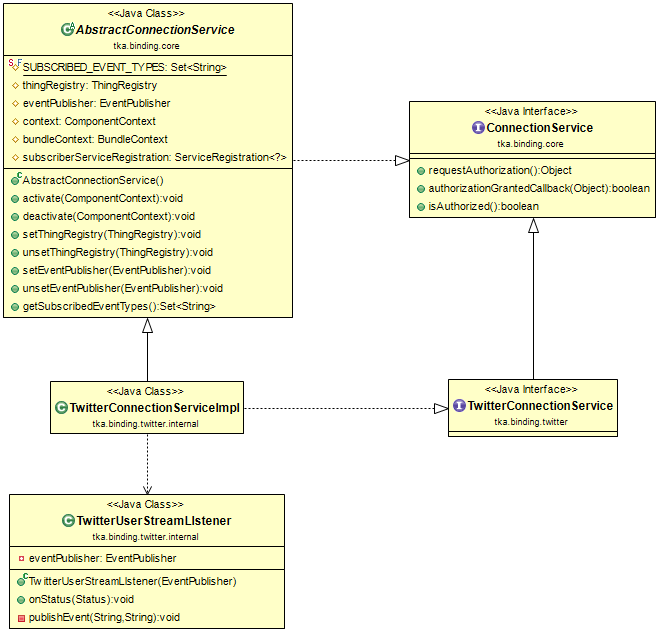
\includegraphics[width=\textwidth]{bilder/ConnectionService}
	\caption{Die Struktur einer Verbindung mit Besipielimplementierung für Twitter}
	\label{fig:connectionservice}
\end{figure}

\subsubsection{ConnectionService}
Die ConnectionService Schnittstelle bietet drei wesentliche Methoden, die bei der Authentifizierung relevant sind. Per \textit{requestAuthorization} teilt der Nutzer mit, dass er wünscht, die Anwendung mit einem seiner Webservice-Accounts (beispielsweise Twitter) zu verknüpfen. Daraufhin bekommt er in der Regel eine URL geliefert, über die er dies umsetzen kann. Die PIN, die er auf diese Weise erhält, teilt er über den \textit{authorizationGrantedCallback} der Anwendung mit. Schließlich lässt sich über \textit{isAuthorized} stets abfragen, ob die Anwendung bereits über die benötigten Zugriffsrechte verfügt. Im Rahmen dieser Arbeit wurde entschieden, sich auf die tatsächliche Unterstützung nur eines Accounts einer Art zu beschränken, obwohl die generische Struktur geeignet ist, um beliebige Mengen von Accounts zu verwalten.

\subsubsection{AbstractConnectionService}
Der AbstractConnectionService bietet eine Reihe von unterstützenden Funktionalitäten, die in der Regel von den Bindings benötigt werden. Hierzu gehört unter anderem die Beziehung des \textit{ThingRegistry}- und \textit{EventPublisher}-Services aus dem System, sowie die eigene Registrierung als \textit{EventSubscriber}. Die ThingRegistry wird benötigt um entsprechende Things im System zu registrieren, nachdem die Autorisierung erfolgreich abgeschlossen ist. Über den EventPublisher publizieren die konkreten Listener (z.B. TwitterUserStreamListener) die Zustandsänderungsevents (mehr dazu in Sektion \ref{sec:bindings_impl}). Als EventSubscriber registriert sich ein ConnectionService um auf Änderungen von Things im System entsprechend reagieren zu können. Beispielsweise, falls ein Thing gelöscht wird, muss auch der zugehörige Listener entfernt werden.\\



Jedes Binding enthält eigene Implementierungen der oben genannten Schnittstellen, die die Besonderheiten des konkreten Webdienstes berücksichtigen. Diese Implementierungen werden außerdem als Services in OSGi registriert, damit über die Benutzeroberfläche die Authentifizierung umgesetzt werden kann.


\subsection{FLASH Erweiterungen}
Das \textit{tka.automation.extension} Bundle registriert im System einige gemeinsamen Services, die von anderen Bundles genutzt werden. Unter anderem wird hier ein neuer Event-Typ registriert: Das \textit{FlashEvent}. Die implementierten Bindings publizieren alle Events dieses Typen, mit unterschiedlichen Topics und Payloads. Dies erlaubt es zu vermeiden, dass jedes Binding seine eigenen Event-Typen deklarieren muss. 


\section{Bindings}
\label{sec:bindings_impl}
Die Bindings sind wie in Sektion \ref{esh:bindings} erläutert aufgebaut. Es wird stets ein neuer Thing-Typ über die \textit{thing-types.xml} im System registriert. Die Anzahl der unterstützten Channels hängt dabei vom jeweiligen Webservice ab.

Jedes Binding integriert einen eigenen Webservice und fügt, sofern notwendig, spezielle Trigger und Actions dem System hinzu. Diese Module erlauben es die Interaktion mit diesen Services über die ESH Rule Engine sinnvoll zu automatisieren.

Alle Bindings haben gemeinsam, dass sie bei den respektiven Webdiensten zunächst registriert werden müssen. Dabei erhalten sie ein Token, mit dem sie sich gegenüber dem Dienst bei Aufrufen identifizieren. Wie komplex dieser Ablauf ist, hängt vom jeweiligen Service ab.

\subsection{Anbindung von Twitter}
Das Twitter Binding fügt dem System Things des Typs \glqq twitter\grqq{} hinzu. Es wird derzeit der Channel \glqq status\grqq{} unterstützt. Dies bedeutet, dass es möglich ist über die Rule Engine den aktuellen Status des Nutzers über Regeln zu manipulieren. Die entsprechende Logik ist in dem \textit{TwitterHandler} und der \textit{TwitterAction} hinterlegt. \\

Der \textit{TwitterHandler} ist ein ThingHandler, der konkrete (String-)Commands erhält und dafür verantwortlich ist den Twitter-Status des Nutzers entsprechend zu aktualisieren.  Hierzu liest er sich die Zugriffsdaten aus der Thing-Konfiguration aus und teilt Twitter mit, was geschehen soll.\\

Die \textit{TwitterAction} ist dafür verantwortlich die konkreten Commands zu erzeugen und an den entsprechenden TwitterHandler zu vermitteln. Hierfür erwartet sie eine Reihe von Konfigurationsparametern, die benötigt werden, um eindeutige Befehle zu erstellen. In Tabelle \ref{table:io} ist aufgeführt, welche Eingabeparameter das Modul erwartet.\\

Umgekehrt ist das Binding in der Lage auf viele Zustandsänderungen des Accounts zu reagieren. Die konkrete Logik hierfür ist im \textit{TwitterUserStreamListener} implementiert. So werden unterschiedliche Events publiziert, wenn

\begin{enumerate}
\item sich ein Status, dem der Nutzer auf Twitter folgt, ändert. In diesem Fall wird der neue Status im Payload des Events gespeichert.
\item ein Status sich ändert und Medien (z.B. Bilder) enthält. In diesem Fall wird für jedes Medium ein eigenes Event publiziert, dass die Medien-URL enthält.
\item der Nutzer eine Nachricht erhält. Der Text der Nachricht wird im Payload hinterlegt.
\item viele weiter Ereignisse eintreffen.
\end{enumerate}
 
Falls ein bestimmtes Szenario nicht abgedeckt ist, lässt sich der \textit{TwitterUserStreamListener} entsprechend erweitern.\\



Bei der Interaktion mit Twitter kommt die Twitter4J-Bibliothek\cite{twitter4j} zum Einsatz. Dabei handelt es sich um eine leichtgewichtige Java-Bibliothek, ohne zusätzliche Abhängigkeiten, die die Twitter API 1.1 komplett unterstützt. Sie assistiert zusätzlich bei dem OAuth Prozess. 

Die Twitter4J-Bibliothek ist auch als OSGi Bundle verfügbar.




\subsubsection{Überblick über die relevanten Trigger, Conditions und Actions}
\begin{table}[h]
\centering
\begin{tabular}{l|c|r}
	\textbf{Modul Name}  & \textbf{Eingaben} & \textbf{Ausgaben} \\
	GenericEventTrigger  & -        			&  <triggerId>.event   \\ 
    EventCondition		&	event   			&	-\\
    TwitterAction		&	event [itemName, message]	& 	-	\\
    DropboxAction		&	event [itemName, directory, mediaUrl]	& - \\
    EmailAction			&	event [to, subject, message]	& -\\
    ItemPostCommandAction	& itemName, command	& - \\
\end{tabular}
\caption{Eingaben und Ausgaben der relevanten Trigger, Conditions und Actions}
\label{table:io}
\end{table}

In der Tabelle sind die Eingaben und Ausgaben von wichtigen Auslösern, Bedingungen und Aktionen aufgeführt. Zu beachten ist, dass die Eingaben sowohl über den Kontext übergeben, als auch direkt in der Konfiguration der konkreten Instanz fest definiert werden können. Dies erlaubt es sowohl statische als auch generische Regeln zu definieren. Falls Parameter fehlen sollten, wird die konkret betroffene Aktion nicht ausgeführt, der gesamte Ausführungsprozess wird nicht unterbrochen.

\subsection{Integration von Dropbox}
Das Bundle \textit{tka.binding.dropbox} ist analog zu \textit{tka.binding.twitter} aufgebaut. Es wird der neue Thing-Typ \glqq dropbox\grqq{} mit dem Channel \glqq folder\grqq{} im System registriert. Über diesen Channel gibt es die Möglichkeit neue Dateien in die Dropbox hochzuladen. \\

Der \textit{DropboxChangesTracker} übernimmt die Rolle des \textit{TwitterUserStreamListeners}. Er überprüft alle 5 Sekunden den Inhalt der Dropbox und publiziert Events für sämtliche Änderungen.\\

Über die \textit{DropboxAction} lassen sich neue Dateien automatisch in die Dropbox hochladen. Beispielsweise kann eine Regel erstellt werden, die mit Hilfe eines GenericEventTriggers auf vom Twitter-Binding publizierte (Medien-)Events reagiert und daraufhin über die Medien-URL die Datei an einem spezifizierten Ort speichert.\\

Bei der Interaktion mit dem Webservice kommt die vom Hersteller angebotene Dropbox SDK zum Einsatz. Dabei handelt es sich um eine Java-Bibliothek, die den Entwickler bei der OAuth-Authentifizierung und der gesamten Interaktion mit Dropbox (Hochladen und Löschen von Dateien, etc.) unterstützt. 

Die Dropbox SDK wurde mithilfe des bnd-Tools\cite{bnd} zu einem OSGi-Bundle umgewandelt. Dabei stellte sich heraus, dass sie Abhängigkeiten auf eine Reihe von Android Bibliotheken besitzt. Nach weiterer Recherche ließen sich diese Abhängigkeiten mithilfe des bnd-Tools auf optional umstellen, wonach die SDK problemlos in der OSGi Umgebung eingesetzt werden konnte. 


\subsection{Das Wetter Binding}
Das \textit{tka.binding.weather} Binding weist sowohl Gemeinsamkeiten, als auch Unterschiede zu den bisher vorgestellten Bundles auf. Es handelt sich bei dem Wetterdienst um einen Webservice, der einer regulären intelligenten Wetterstation stark ähnelt. Dadurch ließen sich mehr Funktionalitäten von ESH wiederverwenden, als bei den anderen Diensten.

Gleichzeitig unterscheidet es sich von den bisher vorgestellten dadurch, dass es sich bei dem Webservice um einen öffentlichen Dienst handelt. Das bedeutet, dass ein komplexer Autorisierungsprozess (beispielsweise über OAuth) an dieser Stelle nicht benötigt wird. Dies führt dazu, dass keine eigene Implementierung der in Sektion \ref{impl:core} vorgestellten Schnittstellen notwendig ist. 

Das Binding registriert den neuen Thing-Typen \glqq weather\grqq{} mit den Channels \textit{temperature}, \textit{humidity} und \textit{rain}. 

Da die Zustandsaktualisierung in diesem Fall vergleichsweise simpel verläuft, wurde sie nicht in eine dedizierte Klasse ausgelagert. Stattdessen wurde der ThingHandler um die entsprechende Funktionalität erweitert. Da sich das Wetter von Region zu Region mit sehr unterschiedlicher Geschwindigkeit ändern kann, lässt sich die Aktualisierungsperiode über die Benutzeroberfläche beliebig konfigurieren.


\subsection{Email Funktionalitäten}
Das Bundle \textit{tka.binding.gmail} erlaubt es dem Nutzer Emails zu versenden. Es ist analog zu den bisherigen Bindings aufgebaut. Der Thing-Typ \glqq gmail\grqq{} wird im System registriert und über einen entsprechenden ThingHandler gesteuert. 

Das Binding registriert den Action Typen \textit{EmailAction}, über den der Nutzer angeben kann, an wen eine Email mit den gewählten Informationen gesendet werden soll. Die Email wird von einer anwendungsinternen Google Mail\cite{gmail} Adresse \textit{noreply.flash.ma@gmail.com} über einen öffentlichen SMTP Server versandt.


\subsection{Integraiton von Philips Hue}
Die Integration von Philips Hue Geräten ist insofern für diese Arbeit relevant, als dass Hue Lampen im Rahmen der Evaluation (Kapitel \ref{chap:eval}) eingesetzt werden. Ein entsprechendes Binding ist seitens von Eclipse SmartHome bereits exemplarisch implementiert. Es ermöglicht die Philips Hue Bridge und eine Reihe von unterstützten Lampen zu steuern. Zusätzlich wird automatisches Entdecken und Einbinden dieser Geräte über Universal Plug and Play (UPnP) unterstützt.


\section{Benutzeroberfläche}
Die Benutzeroberfläche ist komplett im Bundle \textit{tka.flashui} realisiert. Das Bundle ist von den Bindings los gekoppelt - es nutzt einige der von ihnen bereitgestellten Services um eine rudimentäre, aber dennoch voll funktionsfähige GUI bereitzustellen. Es ist jederzeit möglich diese Benutzeroberfläche auszutauschen oder weitere Schnittstellen parallel im System zu registrieren.\\

Wie in Sektion \ref{entwurf:gui} angekündigt, wurde die Oberfläche in Form einer Single Page Applikation umgesetzt. 

\subsubsection{Backend}
Seitens des Backends wird vom OSGi Container ein HTTP-Service bezogen, sowie die von den Bundles bereitgestellten konkreten ConnectionServices. Daraufhin wird in Form von Servlets eine Reihe von REST-Schnittstellen definiert, über die verschiedene Informationen aus dem Frontend per AJAX abgefragt werden. 
Auf diese Weise werden Informationen über die aktuell im System verwalteten Rules und Things bereitgestellt. Für jedes Binding gibt es ein eigenes Servlet, das die Interaktion damit (hauptsächlich für die Authentifizierung) ermöglicht. 

%Es wurde entschieden, die Kommunikation mithilfe von Representational State Transfer zu realisieren, da es aktuell als Referenz-Paradigma für die Bereitstellung von intelligenten Geräten im Web gilt \cite{gui_rest}.


\subsubsection{Frontend}
Bei dem Frontend handelt es sich um eine Single-Page-Webanwendung. Es gibt eine HTML-Datei, die ein leeres Grundgerüst für die Seite bietet und eine Reihe von Javascript Dateien, die beim Öffnen der Seite geladen werden. Die verschiedenen logischen Aspekte der  Anwendung werden in separaten JS-Dateien realisiert. Für jedes Binding gibt es ebenfalls eine einzelne JS-Datei, in der die Logik der Zusammenarbeit mit dem konkreten Binding realisiert ist. \\

Das Erweitern der GUI um neue Bindings lässt sich damit auf eine einfache Art und Weise realisieren, ohne existierenden Code ändern zu müssen. Seitens des Backends muss für ein neues Binding eine neue REST-Schnittstelle in Form eines Servlets definiert werden. Das Frontend bedarf	einer lediglich einer weiteren JS-Datei.		\\


\subsection{Funktionalität und visuelle Darstellung}
Die Benutzeroberfläche bietet die Möglichkeit die implementierten Funktionalitäten zur Laufzeit zu konfigurieren. Sie erfüllt alle Anforderungen, die in Sektion \ref{entwurf:gui} festgehalten wurden. Die Oberfläche lässt sich in drei Abschnitte unterteilen, die im Folgenden nacheinander vorgestellt werden.

\subsubsection{Regeln in der Benutzeroberfläche}
In Abbildung \ref{fig:gui_1} sind die mit Regeln zusammenhängenden Funktionalitäten der grafischen Benutzeroberfläche dargestellt.\\

\begin{figure}
	\centering
	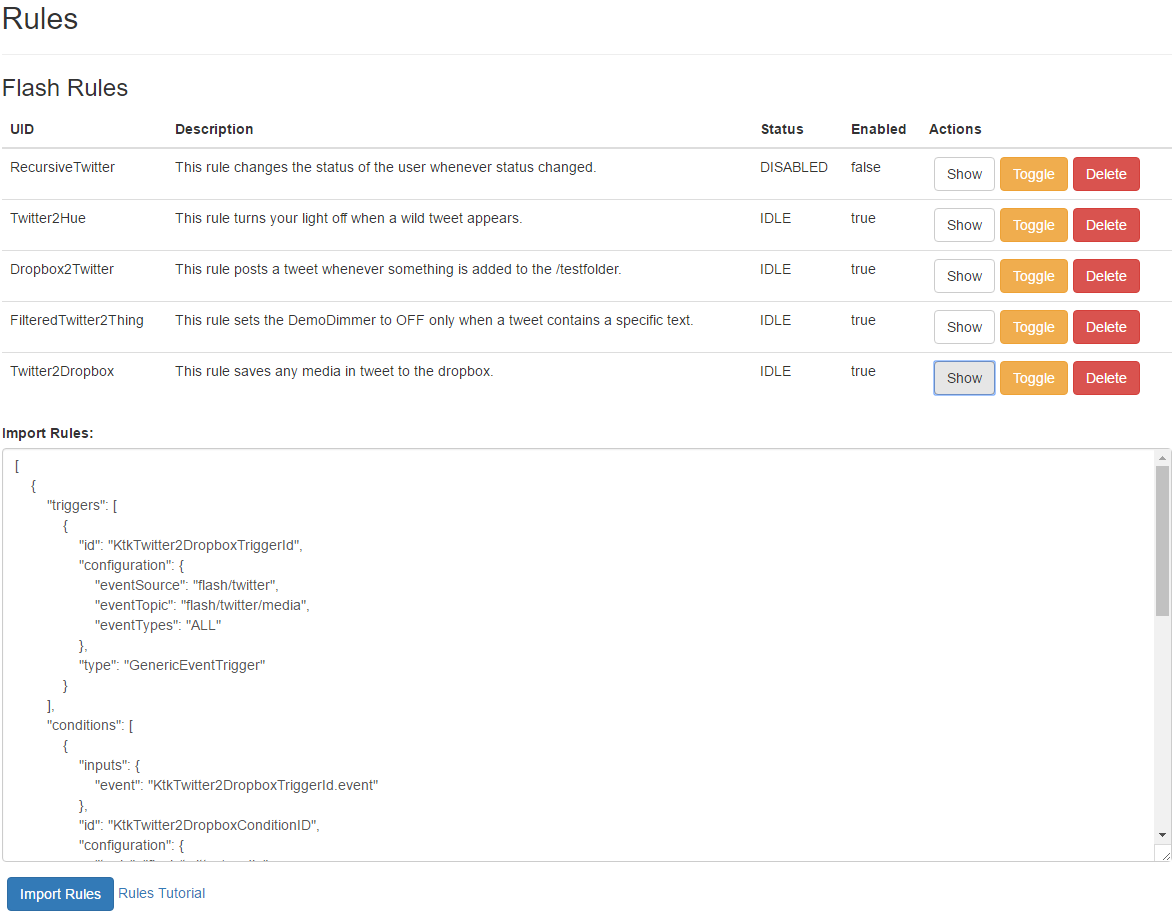
\includegraphics[angle=90, width=\textwidth]{bilder/gui_all4_1}
	\caption{Die Darstellung der Regeln in der Benutzeroberfläche}
	\label{fig:gui_1}
\end{figure}

Im Abschnitt \textit{Rules} werden die aktuell existierenden Regeln in Form einer Tabelle präsentiert. Der Nutzer hat hier die Möglichkeit sich die existierenden Regeln anzuschauen, sie zu (de-)aktivieren und zu löschen. 

Neue Regeln können im JSON-Format konfiguriert und über \textit{Import Rules} an das Backend übermittelt werden. Sie werden daraufhin mithilfe von GSON\cite{gson} zu Rules umgewandelt und dem System hinzugefügt. Auf diese Weise importierte Regeln überschreiben existierende Regeln, die dieselbe Id besitzen.






\subsubsection{Darstellung von Things und Verbindungen}
\label{thing_table}
Die Things und Verbindungen in der Benutzeroberfläche sind in Abbildung \ref{fig:gui_2} dargestellt.\\

\begin{figure}
	\centering
	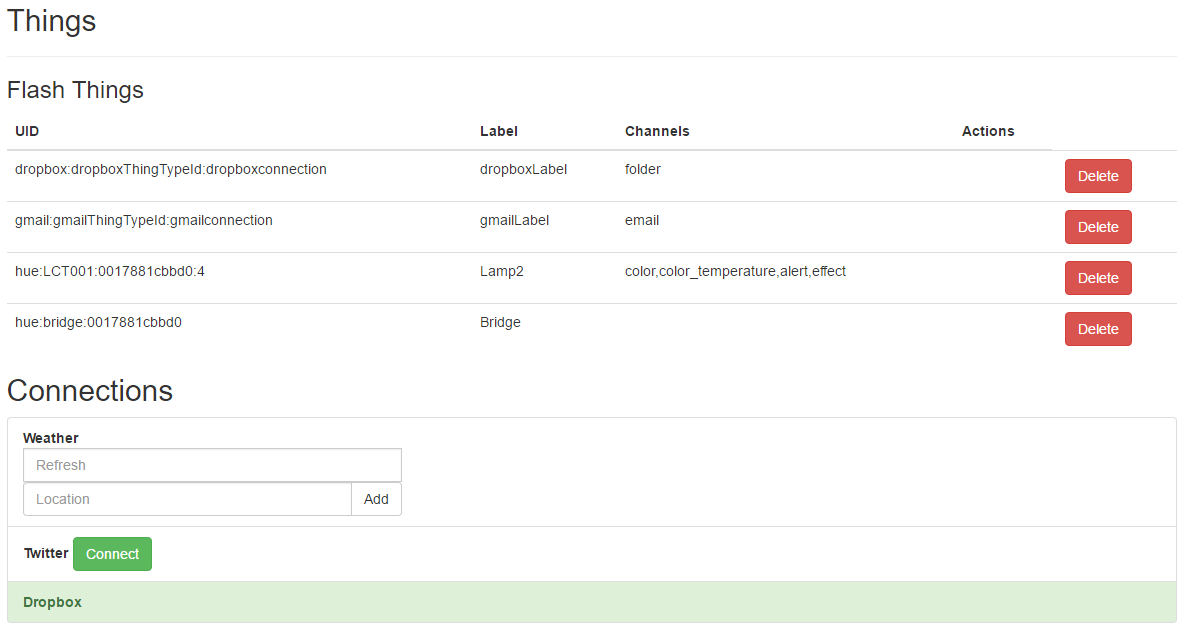
\includegraphics[angle=90, height=\textheight]{bilder/gui_all4_4}
	\caption{Die Darstellung der Things und Verbindungen in der Benutzeroberfläche}
	\label{fig:gui_2}
\end{figure}

Im Abschnitt \textit{Things} sind die aktuell im System vorhandenen Things mit den von ihnen unterstützten Channels zu sehen. Der Nutzer hat hier außerdem die Möglichkeit sämtliche Things zu löschen.\\

Unter \textit{Connections} ist eine Liste mit den unterstützten Webservices zu sehen. Für jeden Webdienst gibt es hier die Möglichkeit die Zugriffsrechte an die Anwendung zu vermitteln (siehe \textit{Connect}-Knopf neben Twitter). Daraufhin wird der Nutzer zu einer entsprechenden URL (wie in Sektion \ref{subsubsec:oauth} erläutert) weitergeleitet. 
Falls der Authentifizierungsvorgang bereits abgeschlossen ist, so wird der Listeneintrag grün hinterlegt und ein entsprechendes Thing in der Thing-Liste angezeigt. 

Da der online Wetterdienst keine Authentifizierung seitens des Nutzers benötigt, kommen OAuth-Weiterleitungen an dieser Stelle nicht zum Einsatz. Stattdessen wird dem Nutzer die Möglichkeit gegeben eine beliebige Anzahl von entsprechenden Things zu konfigurieren und dem System hinzuzufügen.\\

Da die Konfigurations- und Zugriffsdaten ausschließlich im entsprechenden Thing gespeichert werden, ist das Löschen des Things semantisch äquivalent zum Zurückziehen der Berechtigung den betroffenen Dienst im Namen des Nutzers zu verwalten. Auf diese Weise kann der Nutzer seine Accounts von FLASH entkoppeln.


\subsection{Regel Syntax und ihre Mächtigkeit}
Wie in vorherigen Sektionen erläutert, können neue Regeln in JSON deklariert und über die Benutzeroberfläche dem System hinzugefügt werden. Im Folgenden werden anhand einer Beispielregel die vier logischen Abschnitte der JSON-Deklaration erläutert. Die ausgewählte Regel sorgt dafür, dass sämtliche in Tweets hochgeladene Bilder automatisch in einen spezifizierten Dropbox-Ordner kopiert werden.

\subsubsection{Meta-Informationen}
Der erste Teil einer Regel besteht aus den Meta-Informationen, durch die sie eindeutig identifiziert werden kann. In Listing \ref{lmeta} sind die verschiedenen Elemente beispielhaft aufgeführt.

\begin{lstlisting}[language=json,firstnumber=1, caption=Meta-Informationen einer Regel im JSON Format, captionpos=b, label=lmeta]
{
    "uid": "Twitter2Dropbox",
    "name": "Twitter2DropboxRule",
    "description": "This rule saves any media in tweet to the dropbox.",
     "tags": [
        "flash"
    ],
    "visibility": "VISIBLE",
    "configuration": {},
    "configDescriptions": [],
    ...
}
\end{lstlisting}

Wie zu sehen ist, hat jede Regel eine eindeutige \textit{uid}. Eine neu hinzugefügte Regel mit derselben uid überschreiben die bereits existierende. Die Attribute Name, Beschreibung und Tags helfen bei der Filterung und Präsentation der jeweiligen Regel. Die Sichtbarkeit regelt, ob Regeln für den Nutzer einsehbar sind. Schließlich gibt es die Möglichkeit zusätzliche Konfigurationsparameter mit Beschriftungen in die Regel aufzunehmen. Es muss ein entsprechender Handler im System existieren, damit sie auf irgendeine Weise ausgewertet werden.

\subsubsection{Auslöser}
Zusätzlich besitzt jede Regel eine Liste von Triggern. In Listing \ref{l2} ist diese Liste für die Beispielregel dargestellt.
\begin{lstlisting}[language=json,firstnumber=1, caption=Die Liste der Trigger im JSON Format, captionpos=b, label=l2]
{
    ...
    "triggers": [
	     {
	         "id": "KtkTwitter2DropboxTriggerId",
	         "type": "GenericEventTrigger",
	         "configuration": {
	             "eventSource": "flash/twitter",
	             "eventTopic": "flash/twitter/media",
	             "eventTypes": "ALL"
	         }	         
	     }
    ],
    ...
}            
\end{lstlisting}
Wie zu sehen ist, hat die Regel in diesem Fall nur einen einzigen GenericEventTrigger. In der Konfiguration kann angegeben werden, welche konkreten Events ihn auslösen sollen. In diesem Fall sind nur die Events interessant, die ausgelöst werden, wenn ein aktualisierter Status auf Twitter ein Medium enthält.

Es ist möglich, beliebig viele Trigger auf diese Weise zu der Regel hinzuzufügen. Die Ausführung wird dann angestoßen, sofern mindestens einer der Trigger erfüllt ist - es handelt sich dabei also um eine logische \textit{oder}-Verknüpfung. Logische \textit{und}-Verknüpfungen werden von ESH begrenzt durch CompositeTrigger unterstützt, werden aber im Rahmen dieser Arbeit nicht näher behandelt.

\subsubsection{Bedingungen}
Nach den Triggern werden zunächst die Bedingungen evaluiert. Wie diese im JSON-Format aussehen, zeigt Listing \ref{l3}.
\begin{lstlisting}[language=json,firstnumber=1, caption=Die Liste der Conditions einer Regel im JSON Format, captionpos=b, label=l3]
{
    ...
    "conditions": [
        {
            "id": "KtkTwitter2DropboxConditionID",
            "type": "EventCondition",
            "configuration": {
                "topic": "flash/twitter/.*"
            },
            "inputs": {
                "event": "KtkTwitter2DropboxTriggerId.event"
            }           
        }
    ],
    ...
}                   
\end{lstlisting}
Die Beispielregel besitzt nur eine EventCondition. Sie analysiert das Event, das den Trigger ausgelöst hat und vom Trigger in den Ausführungskontext gespeichert wurde. Falls der Topic des Events dem spezifizierten regulären Ausdruck entspricht, so gilt die Bedinung als erfüllt. Ansonsten wird die Ausführung der Regel angehalten, da nicht alle Bedingungen erfüllt sind.

Es ist möglich, eine beliebige Anzahl von Conditions in der Regel aufzulisten. Zu beachten ist, dass sie alle erfüllt sein müssen, damit die Regel ausgeführt wird - es handelt sich um eine logische \textit{und}-Verknüpfung. Es ist derzeit nicht möglich die Conditions über ein logisches \textit{oder} zu verbinden.


\subsubsection{Aktionen}
Schließlich müssen noch die Aktionen einer Regel festgelegt werden. Dies ist in Listing \ref{l4} beispielhaft dargestellt.
\begin{lstlisting}[language=json,firstnumber=1, caption=Die Liste der Aktionen einer Regel im JSON Format, captionpos=b, label=l4]
{
...
"actions": [
  {
	"id": "DropboxActionWohooID",
    "type": "DropboxAction",
    "configuration": {
       "directory": "/testfolder/",
       "itemName": "dropbox_dropboxThingTypeId_dropboxconnection_folder"
    },
    "inputs": {
       "event": "KtkTwitter2DropboxTriggerId.event"
    }
  }
 ]
}            
\end{lstlisting}
Die Regel enthält eine Aktion des Typs DropboxAction. In der Konfiguration wird angegeben, in welchem Ordner in der Dropbox die Dateien gespeichert werden sollen. Der Name des Items stellt sich aus dem Namen des Things und des Channels zusammen. Er kann vom Nutzer aus der Thing-Tabelle (siehe Sektion \ref{thing_table}) ermittelt werden. Schließlich muss angegeben werden, welches Event als Kontext für diese Aktion gelten soll. Dies kann besonders bei Regeln mit mehreren Triggern wichtig sein.

Sämtliche Aktionen, die in einer Regel definiert werden, werden sequentiell abgearbeitet. Dabei ist es möglich für früher in der Sequenz auftretende Aktionen Informationen in den Kontext zu speichern, sodass sie von später ausgeführten Aktionen ausgelesen und berücksichtigt werden. Bei Fehlschlagen der Ausführung einer konkreten Aktion werden die übrigen dennoch weiter ausgeführt.




\subsection{Beispiel für die Zusammenarbeit verschiedener Komponente}

\begin{figure}[h]
	\centering
	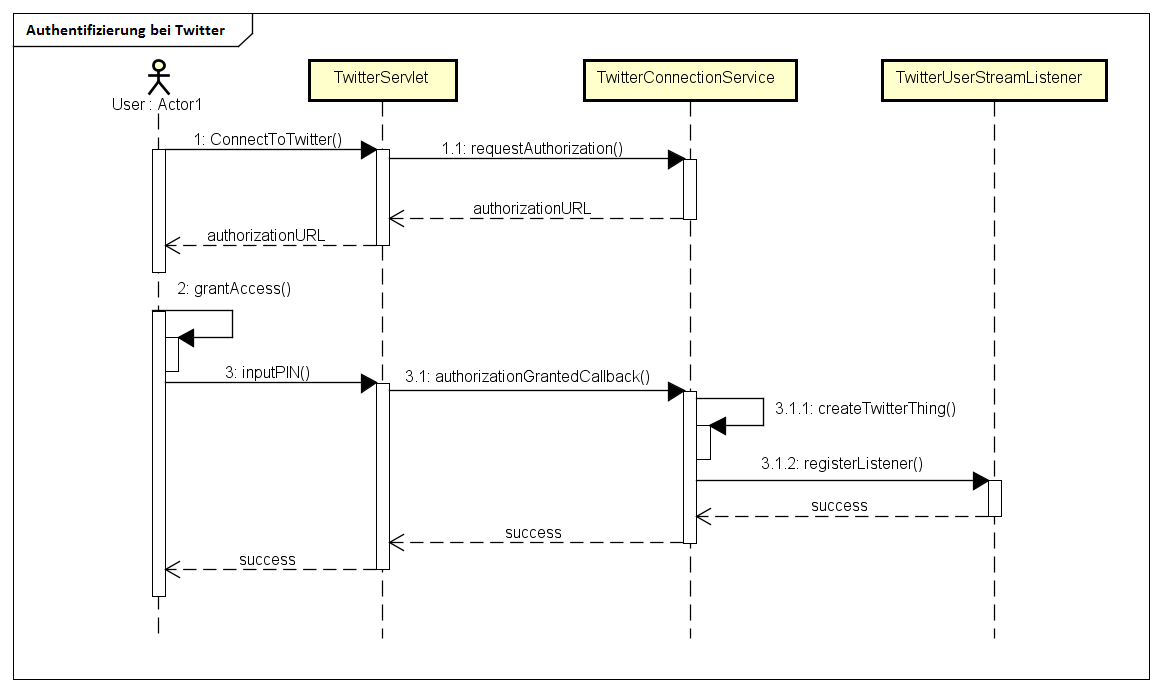
\includegraphics[angle=90, height=\textheight]{bilder/sequenceOAuth}
	\caption{Authentifizierung bei Twitter als Sequenzdiagramm}
	\label{fig:sequenceOauth}
\end{figure}

In Abbildung \ref{fig:sequenceOauth} ist in einem Sequenzdiagramm schematisch dargestellt, wie die Authentifizierung bei Twitter abläuft. Dies soll helfen, die Zusammenarbeit der verschiedenen Komponeneten zu visualisieren.

Der Nutzer entscheidet sich seinen Twitter Account dem Prototypen anzuvertrauen. Daraufhin vermittelt der TwitterServlet ihm eine URL, über die er dies wie in Sektion \ref{subsubsec:oauth} erläutert umsetzen kann. Nachdem die korrekte PIN dem System eingegeben wurde, wird dem System ein neues Thing vom Typ \glqq twitter\grqq{} hinzugefügt und ein entsprechender Listener im System registriert.


\section{Deployment auf dem Raspberry Pi}
\label{impl:deployment}
Das Deployment findet auf einem Raspberry Pi 3 Model B statt. Auf dem Gerät läuft das Betriebssystem \textit{Raspbian} mit installiertem Java 8.

Als Grundlage für die Distribution wird das \textit{Eclipse SmartHome Packaging Sample}\cite{eshsample} verwendet. Es erlaubt es mithilfe von Maven\cite{maven} eine leichtgewichtigen OSGi Container mitsamt einigen der zusätzlich benötigten Services zu bauen. Diese Distribution wurde entsprechend angepasst: 
\begin{enumerate}
\item Weitere notwendige Service-Bundles wurden hinzugefügt. Vor allem bei dem Einbinden von den externen Bibliotheken (Dropbox SDK und Twitter4J) mussten an dieser Stelle zusätzliche Konfigurationen vorgenommen werden.
\item Die eigenen Bundles wurden mithilfe von Maven zu OSGi-Jar-Dateien umgewandelt und zum Deployment hinzugefügt.
\end{enumerate}

Schließlich wurde die Distribution auf dem Raspberry Pi gestartet und und einem umfangreichen Test unterzogen. Die Ergebnisse dieses Tests werden in Kapitel \ref{chap:eval} vorgestellt.

\paragraph{Anmerkung:} Die Distribution kann über das \textit{start.sh} Script gestartet werden. Die Benutzeroberfläche ist unter \textit{http://localhost:8080/flash/index.html} erreichbar.

\section{Fazit}
Die Implementierung wurde entlang des in Kapitel \ref{chap:entwurf} definierten Entwurfs umgesetzt. Sie ist generisch aufgebaut und lässt sich leicht um neue Funktionalitäten erweitern.

\chapter{Evaluation}
\label{chap:eval}
In diesem Kapitel wird die entstandene Implementierung gegen die Anforderungen verglichen und das Ergebnis evaluiert.

\section{Erfüllte Ziele}
Alle formalen Anforderungen, wie sie in Sektion \ref{sec:anforderungen} festgehalten sind, wurden erfüllt. Der Demonstrator läuft on-premise auf dem Raspberry Pi und verwaltet sämtliche Daten lokal. Es ist möglich komplexe Szenarien (Multi Event- und Action-Rules, Kontextweitergabe zwischen den Modulen, etc.) zu definieren, wobei intelligente Geräte mit Webdiensten frei zusammengefügt werden können. Dies ist möglich, da die integrierten Webservices ebenfalls als \textit{Things} im System abgebildet sind. Schließlich ist eine Benutzeroberfläche vorhanden, die es dem Nutzer erlaubt zur Laufzeit neue Szenarien zu erstellen, zu editieren und zu löschen.

\section{Vergleich mit Smart Home}
Bei dem entwickelten Demonstrator handelt es sich um eine klassische Smart Home Lösung, die auf \textit{Eclipse SmartHome} basiert und um weitere Funktionalitäten angereichert wurde. Dadurch verfügt er  über alle üblichen Funktionalitäten, die in einem Smart Home enthalten sind - er ist in der Lage ausgewählte intelligente Geräte direkt anzusteuern und in Szenarien zu automatisieren. 

\section{Vergleich mit webbasierten Task Automation Services}
%Es ist zu beachten, dass es sich bei IFTTT um einen Cloud-Service handelt. Dadurch hat es keine Möglichkeit intelligente Geräte im Haus zu steuern, sofern diese nicht über eine vom Hersteller bereitgestellte Webschnittstelle verfügen.

%In IFTTT ist es nur möglich simple Szenarien auf eine einfache Art und Weise zu definieren. Hierbei handelt es sich um sogenannte \glqq if this than that\grqq{} Szenarien, die über jeweils nur einen Trigger (\glqq this\grqq) und eine Action (\glqq that \grqq) verfügen. Der Demonstrator hingegen erlaubt es komlexe Event-Condition-Action-Regeln zu definieren.

Einen Einblick, wie sich der entstandene Demonstrator in die aktuell existierenden Task Automation Services eingliedern lässt, bietet Abbildung \ref{fig:eval0}. Wie zu sehen ist, gibt es Verbesserungen in vielen Aspekten gegenüber anderen Lösungen. Gegenüber den webbasierten TAS grenzt sich FLASH vor allem durch seine Fähigkeit ab intelligente Geräte direkt anzusteuern, sowie der deutlich mächtigeren Rule Engine ab. Es ist möglich komplexe Szenarien zu definieren, mit beliebig vielen Triggern, Bedingungen und Aktionen. Teile des Szenarios werden sequentiell abgearbeitet und können als Eingabe für spätere Elemente dienen.\\

\begin{figure}
	\centering
	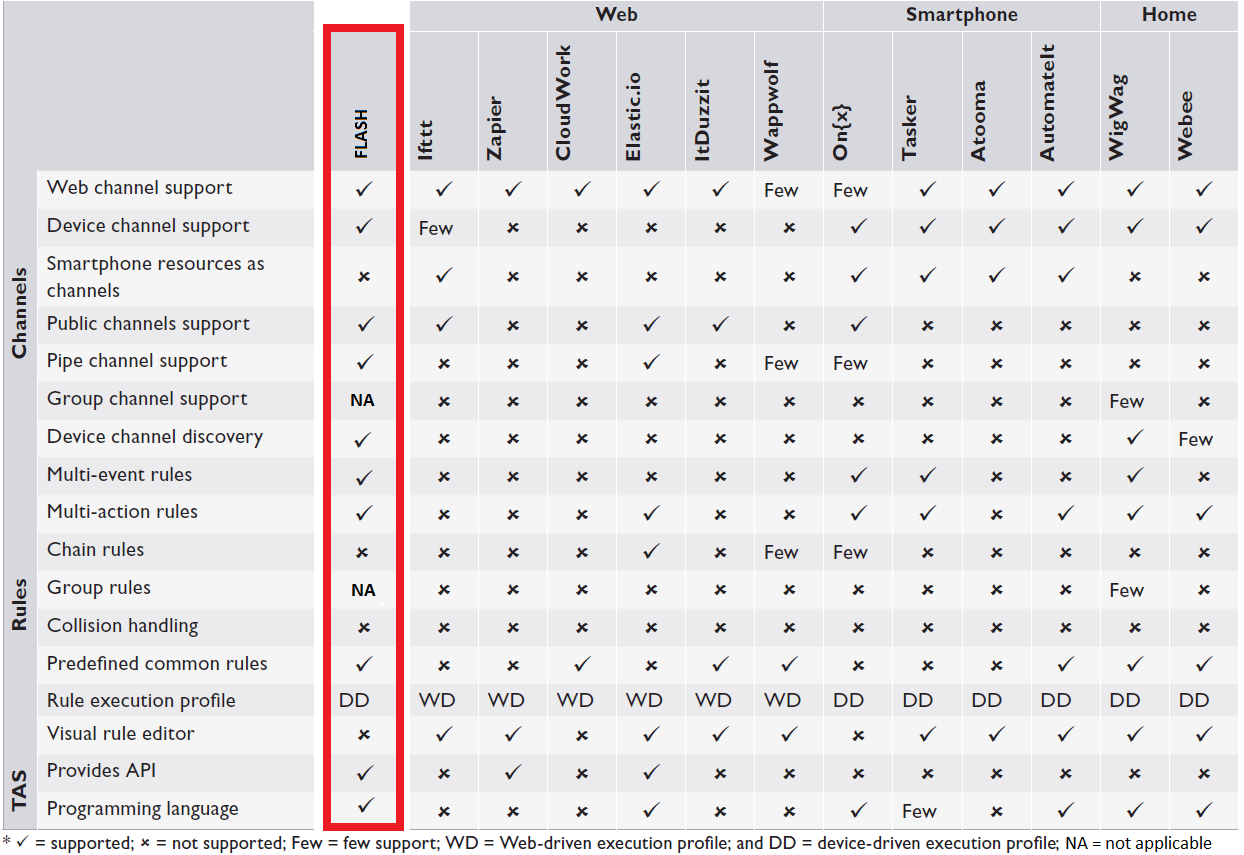
\includegraphics[width=\textwidth]{bilder/TASOverview_eval}
	\caption{Vergleich des Demonstrators mit existierenden Task Automation Services}
	\label{fig:eval0}
\end{figure}


Der entstandene Demonstrator wurde einem umfassenden Test unterzogen, im Laufe dessen Datendurchsatz und Reaktionszeiten gemessen und mit IFTTT und Zapier verglichen wurden. 

\subsection{Kopieren von Dateien in der Dropbox}
Um Durchsatz zu messen, wurde ein Szenario definiert, dass sämtliche Dateien, die in einen bestimmten Ordner in Dropbox hinzugefügt wurden, in einen anderen Ordner in der Dropbox zu kopieren. Zu Beachten ist, dass IFTTT sich auf die Abarbeitung von bis zu 15 Dateien pro Abfrage begrenzt und Dateien, die größer, als 30 MB sind, nicht beachtet. Zusätzlich wird vom Service gewarnt, dass die Ausführung aller Szenarien sich um bis zu 1 Stunde verzögern kann. Diese Tatsache führt zur Streuung, die in den nachfolgenden Grafiken festzustellen ist.

Im Falle von Zapier ist bekannt, dass nur bis zu 5 Zaps pro Abfrage alle 15 Minuten evaluiert werden. Allerdings gibt es keine Einschränkungen in der Anzahl der bearbeiteten Dateien und ihrer Größe. Aufgrund dieses Wissens wurde bei der Evaluation angenommen, dass die durchschnittliche Verzögerung der Ausführung eines Zaps bei 7,5 Minuten liegt.

Der Demonstrator lief auf einem Raspberry Pi 3 Model B, der an einen Router mit VDSL (50 MBit) Verbindung angeschlossen war.

Es wurde geprüft, wie gut die beiden Anwendungen mit einer großen Anzahl kleiner Dateien, sowie mit geringer Anzahl von großen Dateien umgehen können. 

\subsubsection{Zahlreiche kleine Dateien}
Es wurden Mengen von 258 KB großen Dateien gleichzeitig in einen Dropbox Ordner hochgeladen. Es wurden jeweils vielfache von 15 verwendet, da dies die maximale Anzahl von Dateien ist, die IFTTT in einer Abfrage bearbeitet.

Es entstanden die Grafiken \ref{fig:eval1} und \ref{fig:eval2}.
\begin{figure}
	\centering
	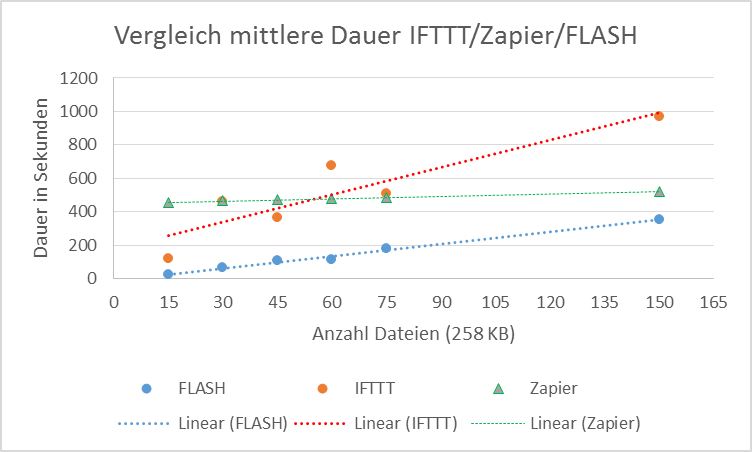
\includegraphics[width=\textwidth]{bilder/vs_mittelwert2}
	\caption{Vergleich des Mittelwerts zwischen IFTTT und FLASH für unterschiedliche Dateimengen}
	\label{fig:eval1}
\end{figure}

\begin{figure}
	\centering
	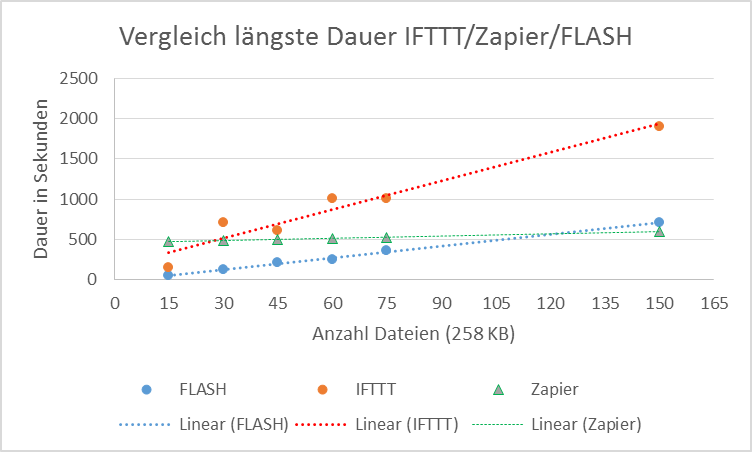
\includegraphics[width=\textwidth]{bilder/vs_laengste2}
	\caption{Vergleich der längsten Dauer (äquivalent zu Gesamtdauer, da ca. 1-2 Sekunden vernachlässigt werden können) zwischen IFTTT und FLASH für unterschiedliche Dateimengen}
	\label{fig:eval2}
\end{figure}

Für die Erstellung von Grafik \ref{fig:eval1} wurde für jede hochgeladene Datei einzeln gemessen, wie viele Sekunden es dauert, bis eine Kopie im Zielordner vorhanden ist. Es wurde anschließend ein Mittelwert gebildet und die Messung mehrmals wiederholt. Schließlich wurde ein gemeinsamer Mittelwert über die gesammelten Werte gebildet und in der Grafik für die verschiedenen Mengen von Dateien dargestellt.

In der Grafik \ref{fig:eval2} wurde analog gehandelt, mit dem Unterschied, dass hier dargestellt ist, was die längste Dauer zwischen hochladen einer Datei und der Bereitstellung der Kopie ist. Da alle Dateien nahezu gleichzeitig hochgeladen werden, kann man diesen Wert auch als Gesamtdauer, bis alle Dateien verschoben wurden, betrachten.

Bei der Messung von IFTTT wurden die berechneten Werte wie gemessen in die Grafik übertragen, da die Verzögerung vor der Ausführung des Applets unbekannt ist und nicht beeinflusst werden kann. Bei Zapier wurde hingegen eine durchschnittliche Verzögerung von 7,5 Minuten angenommen. Da es sich um kleine Dateien handelt und die Zeit, die benötigt wird um eine einzige Datei hochzuladen, vergleichbar klein ist (ca. 1 Sekunde basierend auf den gemessenen Werten) und in Betrachtung der Gesamtzeiten vernachlässigt werden kann, wurde beim Erstellen der Grafik zunächst die kleinste Zeit vom Mittelwert subtrahiert und daraufhin die erwarteten 7,5 Minuten hinzu addiert.

\subsubsection{Große Dateien}
IFTTT ist in der Lage mit Dateien umzugehen, die bis zu 30 MB groß sind. Eine Wiederholung der oben genannten Messung mit 25 MB großen Dateien hat ergeben, dass sich die Ergebnisse  analog verhalten. 

Sowohl der Demonstrator als auch Zapier sind in der Lage mit größeren Dateien umzugehen. Im Test gab es auch bei Verschiebung von 100 MB großen Dateien keinerlei Probleme.

\subsection{Steuern von Lampen bei Tweets}
Es wurde sowohl auf IFTTT als auch auf dem Demonstrator ein Szenario erstellt, dass bei jedem Tweet eine Philips Hue Lampe ausschaltet. Anschließend wurde gemessen, wie lange es dauert, bis die Lampe tatsächlich ausgeschaltet wird, nachdem der Tweet veröffentlicht wurde. Dabei steuert ITTTT die Lampe über die von Hue bereitgestellte Webschnittstelle an, während der Demonstrator das Gerät über WLAN bedient.

Es hat sich ergeben, dass die Reaktionszeit des Demonstrators stets unter einer Sekunde lag, während die Schaltung durch IFTTT eine sehr variable Dauer aufwies. Die schnellste Reaktionszeit lag bei ungefähr 10 Sekunden.

Zapier wurde in diesem Szenario nicht betrachtet, da es die Steuerung von intelligenten Geräten über vom Hersteller bereitgestellte Webdienste nicht unterstützt.


\subsection{Auswertung}
\subsubsection{Vorteile}
Aus den Messungen hat sich gezeigt, dass der Demonstrator IFTTT und Zapier in vieler Hinsicht deutlich voraus ist. Dadurch, dass er sich im Hause des Nutzers befindet, ist er in der Lage mit Geräten direkt zu kommunizieren, was der Grund für merklich bessere Reaktionszeiten in Szenarien, die intelligente Geräte im Haus betreffen, ist.\\

Auch in Szenarien, die nur Web-basiert sind und viel Download/Upload-Volumen mit sich ziehen, hat sich der Raspberry Pi als überlegen erwiesen. Dies lässt sich dadurch erklären, dass es sich bei dem Demonstrator im Gegensatz zu IFTTT und Zapier um ein dediziertes Gerät handelt, dass nur einen konkreten Nutzer bedient. Dies führt auch dazu, dass er keine arbiträren Eingrenzungen besitzt, wie z. B. die Begrenzung der Dateigröße.

Interessant ist, dass sofern Zapier keine Verzögerungen bei der Ausführung von Zaps hätte, es einen höheren Datendurchsatz aufweisen würde. Negativ an Zapier aufgefallen ist, dass es, falls es eine große Anzahl von Dateien (z. B. 150) in einem Zap bearbeiten soll, zunächst den Nutzer um eine Bestätigung bittet. Diese Bestätigung muss jedes Mal manuell erteilt werden, was die Einsatzmöglichkeiten von Zapier eingrenzt. \\

%\paragraph{Anmerkung:} Es ist zu beachten, dass diese Messung mit einem 50 MBit/s Internetanschluss erstellt wurde. Langsamere/schnellere Verbindungen könnten die Messungen entsprechend beeinflussen.\\

Schließlich ist der Raspberry Pi aus einer Datenschutzperspektive dem Cloud-Service zu bevorzugen, da sämtliche Zugriffsdaten nur lokal auf dem Gerät gesichert werden.

\subsubsection{Nachteile}
Negative Aspekte des Demonstrators sind Konsequenz der Tatsache, dass es sich dabei um eine on-premise Lösung handelt. Sämtliche Szenarien, die Webdienste automatisieren, funktionieren nur solange eine Internetverbindung  vorhanden ist. Sollte sie ausfallen, bleiben nur die charakteristischen Smart Home Funktionalitäten erhalten. In diesem Aspekt ist IFTTT dem Demonstrator voraus, da die Ausfallsicherheit in einem Rechenzentrum gegenüber der eines herkömmlichen Heimanschlusses weit überlegen ist.

Umgekehrt ist natürlich zu bedenken, dass bei einem Ausfall des Heimanschlusses auch IFTTT nicht mehr in der Lage sein wird, die hausinternen Geräte über die vom Hersteller bereitgestellten Web-Schnittstellen zu steuern. \\

Die Tatsache, dass sämtliche Zugriffsdaten auf Accounts des Users ausschließlich lokal auf dem Gerät vorhanden sind, zieht mit sich, dass im Falle eines Ausfalls (z. B. Hardware-Fehler) sämtliche Daten verloren gehen können. Dies könnte dazu führen, dass sämtliche Geräte, Dienste und Szenarien nach einer Reparatur komplett neu aufgesetzt werden müssten.



\section{Eclipse SmartHome und Quellcode}
\subsection{Positive Aspekte}
Im Laufe der Arbeit ist klar geworden, dass das Eclipse SmartHome Framework sich gut als Grundgerüst für unterschiedlichste Lösungen handelt. Die sehr generische Struktur des Frameworks hat es ermöglicht, die im Rahmen der Arbeit implementierten Funktionalitäten nahtlos in das Gesamtkonstrukt zu integrieren. 

Dies, sowie OSGi im Allgemeinen, ermöglicht es weitere Funktionalitäten (z. B. weitere Webdienste) der Anwendung hinzuzufügen, ohne bereits existierenden Code ändern zu müssen. Dank der Option, Szenarien im JSON-Format zu definieren, ist es sogar begrenzt möglich, neu hinzugefügte Webdienste in Regeln zu automatisieren, ohne die Benutzeroberfläche anzupassen.

\subsection{Negative Aspekte}
\subsubsection{Eclipse SmartHome}
Negativ aufgefallen ist die mangelnde Dokumentation von ESH, die den Einstieg in das Framework deutlich erschwert. Verstehen der einzelnen Funktionalitäten bedarf der Betrachtung des Quellcodes, wobei relevante Stellen unter den mehr als hundert Bundles erst noch identifiziert werden müssen. 

Eclipse SmartHome befindet sich derzeit noch auf Version 0.9.x und wird aktiv weiterentwickelt. Dies hat unvermeidbar dazu geführt, dass an einigen Stellen der Code nicht fehlerfrei ist. Im Laufe der Implementierung mussten an mehreren Stellen Bugs zunächst ausfindig gemacht und danach behoben werden.

\subsubsection{Quellcode}
Vor allem der Mangel eines visuellen Regeleditors begrenzt derzeit die Nutzungsmöglichkeiten des Demonstrators. Zwar ist es möglich, Szenarien zur Laufzeit zu editieren, so bedarf dies dennoch Kenntnissen von JSON, sowie den existierenden Event-Typen, sowie der Eingaben und Ausgaben von Triggern, Bedingungen und Aktionen.

\section{Fazit}
Die Implementierung erfüllt alle explizit definierten Anforderungen an die Funktionsweise und weist deutliche Verbesserungen in wesentlichen Aspekten gegenüber der Konkurrenz auf. Sie lässt sich leicht um neue Elemente und Funktionalitäten erweitern.


\chapter{Zusammenfassung}
\label{chap:ausblick}

\section{Zusammenfassung}
Hier eine Zusammenfassung




\section{Ausblick}
Hier ein Ausblick

Es hat sich gezeigt, dass die notwendige Hardware durch eine typische Smart Home Base bereits gegeben ist. Auch was den Software Aspekt betrifft, sind viele notwendige Elemente bereits vorhanden. Es ist daher etwas verwunderlich, dass bis dato weder die proprietären noch die open source Smart Home Lösungen die Automatisierung von Webdiensten ermöglichen. 

Diese Tatsache lässt sich zum Teil durch die sehr starke Fragmentierung des Marktes erklären. Typische kommerzielle Smart Home Lösungen unterstützen nur einen kleinen Bruchteil aller existierenden intelligenten Geräte und priorisieren diesen Aspekt, wenn es um die Weiterentwicklung geht. Dennoch lässt sich vermuten, dass in Zukunft, nachdem sich die IoT Landschaft stärker standardisiert hat, die Integration von Webservices in Smart Home etablieren wird.

% Anhang
\appendix
% anhang.tex
\chapter{Weitere Informationen}
Der Quellcode der Implementierung befindet sich auf der mit der Arbeit abgegebenen CD.
% Abbildungsverzeichnis
\listoffigures
\addcontentsline{toc}{chapter}{Abbildungsverzeichnis}
\cleardoublepage
% Algorithmenverzeichnis
%\listofalgorithms
%\addcontentsline{toc}{chapter}{Algorithmenverzeichnis}
%\cleardoublepage
% Literaturverzeichnis
\bibliographystyle{gerplain}
\bibliography{literatur/diplom}
\addcontentsline{toc}{chapter}{\bibname}
% Erklaerung
\thispagestyle{myheadings}
\markboth{}{ERKLÄRUNG}
\addcontentsline{toc}{chapter}{Erklärung}
% erklaerung.tex
\cleardoublepage
\normalsize
Hiermit versichere ich, dass ich die vorliegende Arbeit selbstständig verfasst habe und keine anderen als die angegebenen Quellen und Hilfsmittel verwendet sowie Zitate kenntlich gemacht habe.\\\\
Dortmund, den \today \\\\\\\\
Konstantin Tkachuk
% EOF
\cleardoublepage
\end{document}

